%!TEX root = project.tex

\chapter*{About this project}
\paragraph{Abstract}

This project aims to offer a platform for players to create, manage and compete in competitive online matches. The system is a web application where a user can interact with to create and manage games .\newline The demand for this application is due to how inconvenient it is for an individual to manage custom matches, determining which player goes on what team is time-consuming and very inefficient. This application will automate the process of deciding which player goes on which team through matchmaking. A point system and leaderboard are also provided to produce a competitive environment. How players gain points depends on the outcome of a match and the skill level of their opponents. Users will be able to create an account and log in, allowing them to use the system by viewing and joining public matches or creating their own match for others to join. I hope to develop a cohesive and robust system with a fluent user interface that aims towards people who enjoy a competitive setting and want an extra layer to their gaming experience.
\paragraph{Authors}
Ethan Horrigan


\chapter{Introduction}
In recent years, the competitive online gaming industry (esports) has seen a substantial rise in popularity. \cite{sjoblom2019esports} The estimated global esports audience in 2017 was previously estimated at 335 million people, generating revenue of more than \$900 million with an expected increase of more than \$1600 million in 2021. Yuri Seo and Sang-Uk Jung \cite{seo2016beyond} outlined why people play or enjoy watching competitive games, the main factors include entertainment and to gain a better understanding of a game. People who enjoy competitive gaming can often take part in custom matches of their own, commonly referred to as pick-up games; this is when a group of players form teams and play amongst themselves in a friendly competitive setting. The players involved are responsible for picking the teams and rules for these types of games, more often then not, this leads to unfair matches. This project aims to provide a service for players to manage their pick-up game events and handle the process of matchmaking. The matchmaking system will form balanced teams by fulfilling these two characteristics fairness and uniformity: both sides have a relatively equal chance, and there is little variation between the best and worst players in the match \cite{alman2017theoretical}. I will discuss how the matchmaking system works in more detail below. Users can create a schedule, which will allow the users to determine when an event will take place. When a game has ended players are awarded points, the amount of points they receive depends on the skill level of their opponents. A leaderboard system will track the points they have acquired, allowing players to view their performance in these custom matches.
\newpage
To develop this system, I needed to connect various technologies and allow communication between them. I used Angular as the front-end for the application, where I could design the user interface and communicate with the back-end server to display information. I used Flask for the server and API (Application Programming Interface) this controlled the data communication between the database and the web application.
The features included in the web application are a registration system, login system, leaderboards, match creation, matches page and match display. Then the server-side of the app was responsible for the matchmaking and point system algorithms.

\chapter{Summary}
\paragraph{Context:} here I explain how to the idea for the project came about, I highlight the reasons why this application was made and its core uses.
\paragraph{Methodology:} the Methodology section contains how I went about developing the project, an overview of the technologies used and design choices.
\paragraph{Technology Review:} here I explain how the various technologies were implemented in the project. This section contains working examples of algorithms and features. I explain how I developed, tested and deployed this project.
\paragraph{System Design:} I show how the overall system architecture is designed and implemented. I divide the architecture into individual sections and explain the relationships between databases, platforms and deployment services.
\paragraph{System Evaluation:} I discuss how the overall system works, how I tested the system for performance, the outcome of the project and the limitations that I encountered throughout development.
\paragraph{Conclusion:} I summarise the project and evaluation.

\chapter{Context}
The project aims to provide a service for people to create and manage custom matches for online games. These types of games are usually referred to as pick-up games, which are games that are randomly initiated by a group of players. These types of games are not professional style games nor are they casual. They're somewhere in between. The main objective is to create a web application for users to interact where they can sign up and create or participate in custom games, the application will handle the process of matchmaking players to teams and track progress using a point system.
\section{Skill-Based Matchmaking}
The fundamental purpose of skill-based matchmaking is that a game is enjoyable for all participating players. \cite{graepel2006ranking} If the outcome of a match is uncertain, then participating teams have a fair chance of winning. A game is said to be balanced when both sides have an equal opportunity of winning, and there is little variation between the worst and best players on a team. Being paired against opponents with more or less skill-level can ruin the experience for both parties involved \cite{alman2017theoretical}. Therefore, defeating the fundamental purpose of matchmaking. We can determine players skill-levels by supplying every player with a rating which is a measurement of their skill. There are many systems available to decide on a players rating. The Elo system by Arpad Elo which calculates relative skill levels of players in games such as chess. The Glicko2 System \cite{glickman2012example}, which is as an enhancement of the Elo system, intended to measure rating reliability. TrueSkill is another system for rating players; TrueSkill is designed for games with multiple players, such as team games.
The system used in the project is the Elo rating system. The Elo system \cite{pelanek2016applications} was developed initially for rating chess players, now it is commonly used for ranking players in many online games. Players can quickly find his/her ranking in a game using this system. When updating a players rating, it does not increase at a constant rate, the value at which it increases depends on the skill level of its opponent if a player is matched up against someone with a relatively lower rating, then the rating for the player would not increase as much as if he/she was matched against a player of similar rank. In my opinion, this system introduces fairness.\newline
Based off player ratings mentioned above, we can use these ratings to match players in team-based games, I will discuss in further detail on how the matchmaking system was designed in sections below.
The purpose of this platform is because many groups or communities of players like to have competition between each other but, organising these friendly matches can be a nuisance, whether gathering players to form a match or even attempting to balance teams, this is where the matchmaking system comes in with the aim to avoid these time-consuming actions by providing a platform that handles these operations for the user.
\section{Competitive Gaming}
Competitive gaming often referred to as esports, which can be defined as \cite{sjoblom2019esports} “a form of sports where the primary aspects of the sport are facilitated by electronic systems; the input of players and teams, as well as the output of the esports system, are mediated by human-computer interfaces”. In essence, its a competitive way of playing computer games. This can be compared to 'traditional' sports where players compete amongst each other in a competitive environment. Like sports has its types (Football, Rugby etc..), games have its genres (e.g. First Person Shooter, MOBA, Strategy etc..).\newline


This project will focus on providing a platform for players to manage competitive matches for the popular Multiplayer Online Battle Arena (MOBA), League of Legends.\newline

Within the game, players have different game modes which they can play
(Draft Mode and Ranked Mode). Players can receive a rank when playing in ranked mode meaning players are matched up against opponents with similar skill levels. When searching for a game, players join a queue and the system tries to create a lobby of 10 random players of similar skill levels. Custom lobbies can also be created allowing people to form a lobby of players where players ranks are inconsequential. This allows players to have complete control over the lobby (who goes onto what team). My application will manage these custom games through matchmaking instead of people deciding on who goes where which can be a nuisance and inefficient.

\section{Project Objectives}
The project aims to develop a web application allowing users to create and manage their custom game event. The core objective of this project is to try to eliminate the inefficiency and unpredictability of managing player-made games through the use of matchmaking. For the system to be practical, I aim to implement various features to enable users to manage their games effectively.
Users will be allowed to register an account with the application enabling them to decide when matches take place or even participate in events themselves. \hfill \break
I will gather data on the user's in-game information to join with the data of the application to generate relatable information to make the matchmaking system more reliable. When registering, users link their in-game username which is used to gather more information about the player. This information will be updated every time the user logs into the app, ensuring that their details are up-to-date. \hfill \break
Users will be able to create matches and view matches that have been created by other users. With the intention of building a community of like-minded players. \hfill \break
If someone is particularly interested in a game, they can join that match which will add them to a participants list, once this list reaches maximum capacity, teams will be formed based on their ratings. \hfill \break
After a game has ended, players earn points, the amount of points they receive is based on the rating of their opponents. A leaderboard system will enable users to track how much points they have accumulated and also allows them to track their performance. \hfill \break
The project aims to be accessible and easy to understand to ensure a smooth experience for the user. I will discuss in further detail below, on how I designed and implemented this system.



\chapter{Methodology}
\section{Development Methodology}
The development methodology used throughout the development of the project was Extreme Programming (XP), Extreme Programming is an agile software development framework that aims to deliver higher quality software. Similar to most Agile approaches, Extreme Programming allows for releases in short development sprints, XP also ensured that the app was fault-free because of continuous testing. XP follows simplicity and communication. Before development started, project meetings were established with my supervisor; these early meetings consisted of brainstorming and considering project ideas. During this period, I researched various technologies that could provide use throughout project development. Once the objectives of the project were understood, I divided what needed to be done into iterations, each week I met with my supervisor to discuss what part of the project is currently in development and listened to any feedback. This style of development allowed me to stick to the plan and see changes to the application each week.
\section{Testing}
I used various testing techniques throughout the project, unit testing, end-to-end testing and automated testing were among the main testing types I used. I implemented the functionality of client-side elements before conducting tests; therefore, I could test the system as a whole. Jasmine and Karma was the framework used to test the functionality of web components, pythons unittest for back-end unit testing and automated tests for how the application worked at a user level.

\begin{center}    
	
\includegraphics[width=8cm,height=3.3cm,keepaspectratio]{img/Jasmine_and_Karma.png}
\end{center}
Python’s Unittest was used to test server-sided functions ensuring that both HTTP Requests and the Matchmaking algorithm operated as expected.
\begin{center}    
	
\includegraphics[width=8cm,height=3.3cm,keepaspectratio]{img/Unittest.png}
\end{center}
End to end testing (e2e) was used to test the interactions and relationships between the backend and the presentation layer of the application. E2e testing was a great way to ensure that the components of the application worked together cohesively and also the application functioned correctly at a high-level overview. I concluded that unit tests were not sufficient enough, as unit tests only tested isolated elements of my project. I needed to test how the application's components operated as a combination. E2e testing was the best way to accomplish this.
Test cases were generated by scenarios in the following ways:~\cite{bai2001distributed}
\begin{itemize}
	\item (1) Identify the input data that meet the conditions associated with the component based on different testing techniques (e.g. unit tests).
	\item (2) Determine the expected results from input data. 
\end{itemize}
The main way I generated test cases was based on application usage, e.g., one component can be affected by several conditions, and each condition can be satisfied by multiple data. For example, the registration element may have input data such as username, summoner name and password. Therefore, the conditions for this test case include
\begin{itemize}
	\item 1) Valid username; 
	\item 2) Valid summoner name; 
	\item 3) Valid password;
\end{itemize}
The first test case satisfied these inputs and then the second test case took the exact input from the first scenario proving that duplicate usernames cannot be inserted into the database.

\paragraph{}
I also performed Automated Tests when adding new features, this enabled me to conduct tests that I would normally do manually, e.g. testing the login system. I installed Selenium \cite{selenium} as a browser extension and manually recording various tests, I could run these tests whenever I was testing a new feature, this saved a lot of manual typing and navigating which can add up over time.
\section{Project Management and Source Control}
GitHub was used for source control and project management. Initially, I was using Trello for task management but this quickly became complicated to associate updates with unfinished tasks of the project. Therefore I changed the projects task management to GitHub’s Issues section. I posted issues for any viable element that needed to be implemented into the project and when one of these elements were complete I would close the corresponding issue on GitHub. Each issue was categorized with tags depending on the type. These tags include:
\begin{itemize}
	\item To-do: Tasks that have yet to be implemented.
	\item Tests: Types of tests that have been or need to be carried out.
	\item Bugs: Issues or bugs that occurred throughout the project and how they were solved.
	\item In progress: In progress are tasks that are currently being implemented.
	\item Completed: Finished tasks.
	\item Enhancement: When a completed part of the project has been upgraded, changed or removed.
\end{itemize}
This method of task management proved to be a lot more manageable compared to my previous method of using Trello. I could easily compare my current tasks to my commits on GitHub. Anytime I had implemented a significant change or addition to my project, I would perform commit it to through git and push the change.

\section{Technologies Selection Criteria}
\subsection{Front-end}
I used Angular framework for front-end development, Angular is an open-source web application framework led by Google. The reason I opted for Angular is because it provided everything I needed to develop a production-ready web application. Angular uses TypeScript, which is a superset of Javascript \cite{bierman2014understanding}. TypeScript improves JavaScript with a module system, classes, interfaces, and a static type system. This allowed me to develop in a more structured manner. Angular also provides detailed and easy to follow documentation \cite{docsangular}, making life alot easier when learning this framework.
Angular Material is another feature that allows developers to easily integrate UI components. Building the application was done using Angular's ahead-of-time (AOT) compiler \cite{aotc} which converts Angular HTML and TypeScript code into JavaScript code. This meant I could compile my code into one package and then use this package for deployment. A core feature that Angular provided is Two-way data binding, this means that when properties in the model get updated, so does the view (user interface) and when user interface elements get updated, the changes get delivered back to the model.
With the factors discussed, Angular seemed like the right choice for this application.
\subsection{Back-end}
Since I wanted to experience new technologies and had already used the MEAN stack before, I had the option to either use Flask or Django; which are both web application frameworks in Python. A web framework is a combination of packages or modules that make life easier when building scalable, reliable, and maintainable web applications. Frameworks often promote code reuse for common HTTP operations and aim to automate the burden associated with everyday activities performed in web development \cite{rengglib2004seaside}. \hfill \break
I opted for a flask server, I chose flask for multiple reasons, some of them being: it supports all SQL and NoSQL databases, and because I was unsure at the beginning of what database I should use, this feature stood out to me.
Flask classifies as a micro-framework. Micro-frameworks are usually frameworks with little to no dependencies to external libraries \cite{aboutflask}; they lack most of the functionality which is typical to expect in your regular web application framework, for example, they do not provide authentication or authorization. Although this seems like a reason to not use flask, it meant I had creative freedom on what I wanted to add, and I could learn how functions like user authentication or authorization worked by implementing them myself. \hfill \break
\subsection{Database}
The primary development environment used throughout the project was Visual Studio Code, The main reasons why I chose this environment is because it supports browser debugging, Git control, syntax highlighting, intelligent code completion and for its customisability. Both front-end and back-end of the project were developed in this environment.
I used Angular which is an open-source web application framework led by the Angular Team at Google. The reasoning behind choosing Angular is because I wanted the project to be a web application as compared to a hybrid application, Angular seemed to be the most viable framework for this application. Through angular, I could write the functionality of the front-end using typescript, which is then compiled down to javascript. Typescript is more structured then Javascript which I preferred.
When researching options for the database server, the two main options were python and flask or using MEAN stack (Mongo, Express.js, Angular and Node). I wanted the database to be a relational instead of using a NoSQL database, so a NoSQL database did not suit. I also wanted to use a technology that I'm not familiar with. So I opted for Python and Flask.
\par


\begin{figure}
	\centering
	\begin{tikzpicture}[node distance=6cm]
	\node (a) [rect] {Github};
	\node (b) [rect, below of=a] {Server (Flask)};
	\node (c) [oval, right of=b] {Client (Angular)};
	\draw [line] (a) -- (c);
	\draw [line] (b) -- (c);
	\end{tikzpicture}
	\caption{Nice pictures}
	\label{tikz:graphs2}
\end{figure}


\chapter{Technology Review}
\section{Angular}
Angular is an open-source web application framework led by the Angular Team at Google. It is often used for building Single Page Applications (SPA). What is a Single Page Application? In a web application, when you navigate to a different page, the entire page is reloaded, in a SPA, only the view of the content requested is reloaded. SPA provides a fluid experience for the user. A good example of a Single Page Application is Twitter. Since this application is a SPA, navigating between pages was smooth. A constant array of Routes is declared for every component.
\begin{minted}{typescript}
const routes: Routes = [
{ path: 'mypath', component: MyComponent}
{ path: 'mypath2', component: MyComponentTwo}
{ path: 'mypath3', component: MyComponentThree}
];
\end{minted}

\subsection{Why Angular?}

\begin{itemize}
	\item Components
\end{itemize}
Angular allows you to create components that provide functionality, styling and views.

\begin{itemize}
	\item Dynamic Routes
\end{itemize}
I could create unique URLs through Angulars ActivatedRoutes feature. I used this for viewing users profiles and particular match details. The URL parameters could also be accessed.
\newpage Example Button to view a match.
\begin{minted}{typescript}
//Typescript
{ path: 'match/:matchId', component: ViewMatchComponent},
\end{minted}
\begin{minted}{html}
 <!-- HTML -->
<a href="match/{{game.match_uuid}}" class="btn btn-primary">Join</a></li>
\end{minted}

\begin{itemize}
	\item Data Binding
\end{itemize}
Allows accessing of data from Typescript code to the html page view. This eliminates the process of implementing data binding myself.
Example:
\begin{minted}{typescript}
// TypeScript String Variable
myString: string = "Hello, World";

// Data Binding on the HTML Page
{{myString}}
\end{minted}

\begin{itemize}
	\item Testing
\end{itemize}
Angular includes testing frameworks (Jasmine, Karma and Protractor) for e2e testing and unit testing. When creating a new component, A template spec file is also created where test cases for each component can be easily written.

\section{SQLite}
SQLite is an open-source relational database. I used SQLite in the development of the project so I could audition how data was structured for the entire application. Each table went through iterations of changes until I was satisfied with the database schema. SQLite database is stored as a file locally \cite{newman2004sqlite} instead of running as a stand-alone process.
This made it easier to develop a prototype database and understand how data will be interpreted when deploying.
When I finally developed a functioning database I converted to a PostgreSQL production database. This was a smooth transition as both databases were relational. This meant queries didn't change and only how the database connected to the server and had to be changed.

\newpage
\begin{itemize}
	\item Connection to SQLite Database:
\end{itemize}

 \begin{minted}{python}
db_connect = create_engine('sqlite:///dev_database.db')
\end{minted}

\begin{itemize}
	\item Connection to PostgreSQL Database:
\end{itemize}

\begin{minted}{python}
connection = psycopg2.connect(user=user, password=db_password, host=host, port=port, database=database)

cursor = connection.cursor(cursor_factory=RealDictCursor)
\end{minted}
\section{PostgreSQL}
PostgreSQL (Postgres) is a Relational Database Management System (RDBMS). 
\cite{postgresql1996postgresql} Postgres is known for its reliability, data integrity and extensibility. The main reason why I chose Postgres as my production database is because of its extensibility, ensuring my application is scalable for future growth. Postgres also provides concurrency meaning queries can be read in parallel allowing multiple users to use the database at the same time.
\paragraph{Tables:}Matches and Participants both contained a match id primary key, I could access match data from both tables using a match id number. These tables were used in match creation and joining.
\begin{table}[h]
	\centering
	\begin{tabular}{llllll}
		\toprule \\
		match id & match type & match name & date & outcome & admin \\
		\midrule \\
		Row 1.2  & Row 1.2    & Row 1.3    & Row 1.4 & Row 1.5 & Row 1.6\\
		\bottomrule
	\end{tabular}
	\caption{Matches table.}
	\label{table:Matches}
\end{table}
\begin{table}[h]
	\centering
	\begin{tabular}{llllll}
		\toprule \\
		match id & username & summonername \\
		\midrule \\
		Row 1.2  & Row 1.2  & Row 1.3  \\
		\bottomrule
	\end{tabular}
	\caption{Participants table.}
	\label{table:Matches}
\end{table}
\section{PgAdmin and DBeaver}
TALK ABOUT DBeaver
PgAdmin \cite{pgadmin} is a database management tool for PostgreSQL. It simplifies the creation, maintenance, and use of database objects through a user interface. I used pgAdmin for database maintenance and to get a visual representation of data that was stored in my database. I linked the local and deployment PostgreSQL database to pgAdmin making both easily accessible for development.
\section{Heroku}
Heroku \cite{heroku} is a Free Cloud Application Platform. The Flask Server and PostgreSQL Database were both deployed on Heroku. Heroku runs applications in "dynos" which are basically just virtual computers. I created a branch on GitHub specifically for Heroku, so every time I made a new commit to GitHub, Heroku would automatically build. This allowed me to develop alot more efficiently because I did not have to start up the server each time and changes to server were automatically built, deployed and ran on each git push. 
\paragraph{Setup:} to setup Heroku for my server. I had to give it a requirments file, which contains all the servers dependencies. This is so Heroku can set up an enviroment to run the server.
\begin{minted}{text}
riotwatcher==2.7.1
Flask_Cors==3.0.8
Flask_RESTful==0.3.7
psycopg2==2.8.4
SQLAlchemy==1.3.12
numpy==1.17.3
Flask==1.1.1
python_bcrypt==0.3.2
\end{minted}
A Procfile is also made, to let Heroku know how to run the server.
\begin{minted}{text}
web: gunicorn api:app
\end{minted}
\newpage
\section{Firebase}
Firebase \cite{firebase} is a web application development platform. I used Firebase primarly for its Cloud Hosting \cite{peteva2017cloud}. Firebase provided resources for me to deploy and manage my front-end application remotely in a cloud infrastructure. This provided access for public and private end-users.
\paragraph{Setup:}
First, I created a Firebase account and a Firebase App.
I then built my front-end application into one distribution folder (/dist)
\begin{minted}{bash}
ng build --prod --aot
\end{minted}
After building the project, I initialised the Firebase app.
Selecting hosting as the feature setup.
\begin{minted}{bash}
firebase init
\end{minted}
Once the project was finish initialising, I deployed the app.
\begin{minted}{bash}
firebase deploy
\end{minted}
I could then navigate to the deployment url, to view my deployed application.
\section{Cloud Platforms}
Both Heroku and Firebase are types of cloud services;  which can be described as computing services including servers, storage, databases and software which are available for users over the internet aka "the cloud".
Heroku and Firebase are categorised as a Platform as a Service (PaaS); these services allow developers to build and run their software in the cloud. 
PaaS is designed to make it more straightforward for developers to create, run and manage applications, without the need for developers to worry about setting up and maintaining their own infrastructure. These platforms can be accessed from anywhere remotely, making them easily accessible. Both Heroku and Firebase are free to use, allowing developers to host their server and database without additional cost, although they are free they also have options to upgrade meaning they have high scalability. PaaS increases productivity for developers; for example, each time someone wants to access their local server, they would have to set it up and run it and then connect to it. Heroku enables developers to host their server on the cloud, making it readily available for when they need to access it. Instead of focusing on the infrastructure, developers can focus on the applications logic.
\section{Flask}
Flask is a web framework written in Python. I used Flask to develop the projects API. The projects databases and Riot Games API were connected to the flask server. This basically provided communication via CRUD operations between the projects front-end and back-end.
\paragraph{Setup}
\begin{minted}{python}
from flask import Flask, request, jsonify
app = Flask(__name__)
\end{minted}

Example of a GET request to Riot Games API to retrieve players id.
\begin{minted}{python}
def get_account_id(self):
player_details = watcher.summoner.by_name(my_region, self)
return player_details['accountId']
\end{minted}
\newpage
Working example of a GET request to retrieve match details.
\begin{minted}{python}
class GetMatch(Resource):
def get (self, _match_uuid):
cursor = connection.cursor()
query = ("Select match_uuid, match_name, match_type, date, time, admin, outcome from matches WHERE match_uuid =%s")
query_param = [_match_uuid]
 cursor.execute(query, query_param)
columns = [desc[0] for desc in cursor.description]
result = {'games': [dict(zip(columns, row)) for row in cursor.fetchall()]}
return result
\end{minted}


\section{RiotWatcher}
RiotWatcher is a Python wrapper for Riot Games API, RiotWatcher supports a simple rate limiter. This \cite{dealcisco} rate limiter will try to stop you from making too many requests to Riot Games API. I used RiotWatcher to access players in-game data and then store relevant data in my database to be used throughout the project. Here is a working example of retrieving a players ID number and verify if the player exists in Riot Games database.
\begin{minted}{python}
from riotwatcher import RiotWatcher, ApiError

watcher = RiotWatcher(<api-key>)

def get_player_details(self):
	try:
		response = watcher.summoner.by_name(my_region, self)
	except ApiError as err:
		if err.response.status_code == 429:
			print('Too many requests')
	elif err.response.status_code == 404:
		response = "SUMMONER_NOT_FOUND"
	return response
\end{minted}
\newpage
\section{Postman}
Postman \cite{postman} is a platform for Application Programming Interface (API) development. I used Postman to perform CRUD operations (Create, Read, Update, Delete) on Riot Games API and the projects API. I created collections of each request so I could easily test each operation before implementing into the projects front end. When the project was deployed, I ran the same tests but used the projects deployment URL.
\section{Jasmine}
Jasmine \cite{jasmine} is a behaviour-driven development framework for testing JavaScript code. Jasmine is a set of functions that perform unit tests. You give a function and what the result should be. These unit test cases \cite{elbaum2006carving} focuses on the individual components of the project. Jasmine was mainly used to test static components, e.g. buttons, form fields, titles etc..
\paragraph{Example:} validating user input field on the registration component
\begin{minted}{typescript}
fdescribe('RegisterComponent', () => {
	let component: RegisterComponent;
	let fixture: ComponentFixture<RegisterComponent>;	
	beforeEach(async(() => {
	TestBed.configureTestingModule({
		declarations: [ RegisterComponent ],
		imports: [ RouterTestingModule, FormsModule,],
	})
	.compileComponents();
}));

it('should validate username', () => {
	const nameInput = component.registerForm.controls.username;
	
	expect(nameInput.valid).toBeFalsy();
	
	nameInput.setValue('TestName');
	expect(nameInput.valid).toBeTruthy();
});

\end{minted}
 
\section{Karma}
Karma \cite{karmatesting} is a tool which opens a web server that executes source code against test code. The results of each test against each browser are displayed via the command so I can see if the tests passed or failed. Jasmine tests are executed through Karma. Using a configuration file, I can set which testing framework (Jasmine), port, browser and plugins needed to execute Karma.
\paragraph{My Karma Config:}
\begin{minted}{javascript}
module.exports = function (config) {
	config.set({
	 basePath: '',
	 frameworks: ['jasmine', '@angular-devkit/build-angular'],
	coverageIstanbulReporter: {
	 dir: require('path').join(__dirname, './coverage/frontend'),
	 reports: ['html', 'lcovonly', 'text-summary'],
	 fixWebpackSourcePaths: true
	},
	 port: 9876,
	 autoWatch: true,
	 browsers: ['Chrome'],
	 singleRun: false,
	 restartOnFileChange: true
	});
};

\end{minted}

\section{Selenium}
Selenium is a web testing tool which uses scripts to automate tests directly within a browser \cite{holmes2006automating}. I used Selenium for user interface automation testing. Instead of manually testing the UI which is time-consuming and error-prone, I could automate manual tasks through Selenium.

\paragraph{Example:}when implementing the user authentication system, I would have to enter the user details every time I wanted to test its functionality. Using Selenium, I could automate this process by recording each step of logging in with a test set of user details, then anytime I wanted to test the login system, I would execute this script through Selenium's IDE browser extension.
\begin{center}
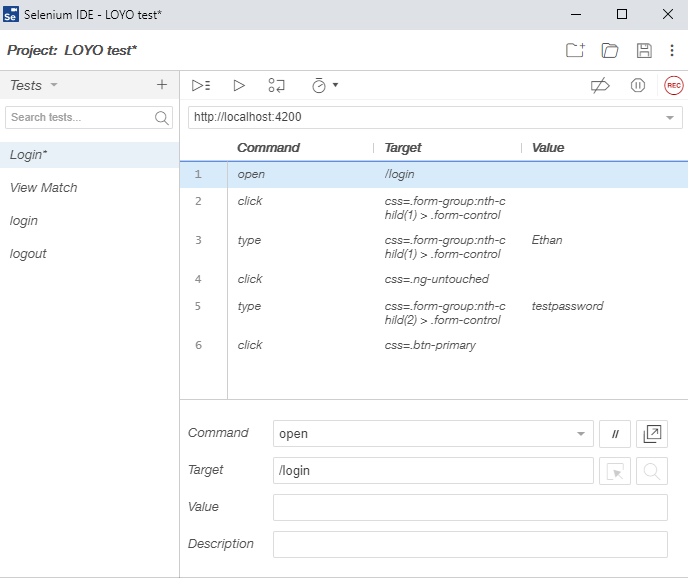
\includegraphics[width=10cm,height=5.3cm,keepaspectratio]{img/Selenium.png}
\end{center}


\chapter{System Design}

\begin{figure}[H]	  
	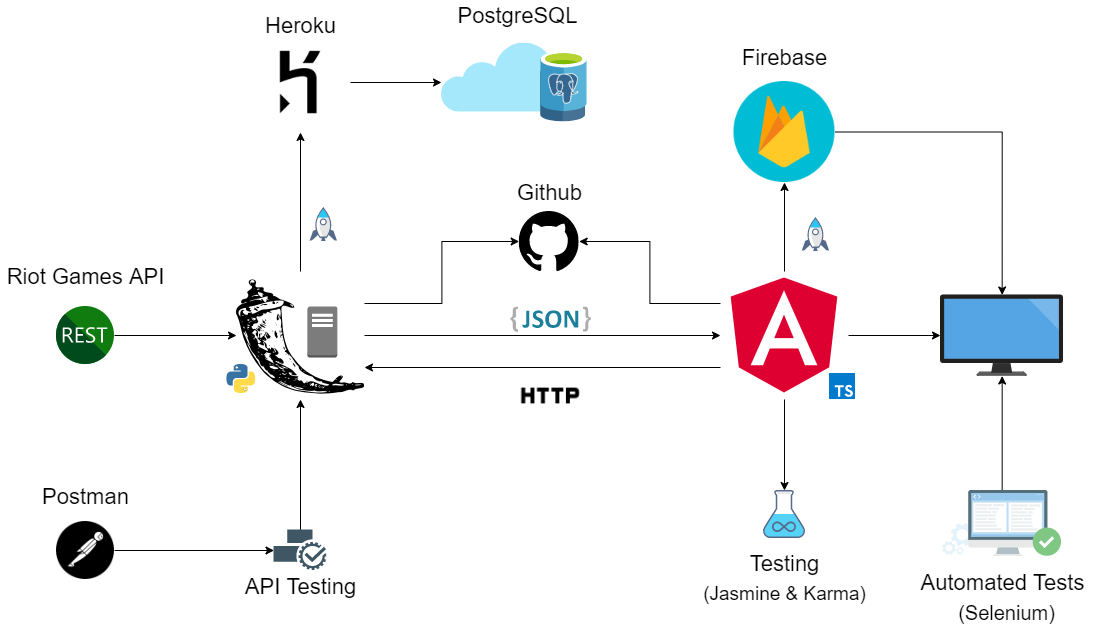
\includegraphics[width=\textwidth,height=\textheight,keepaspectratio]{img/Architecture.png}
	\caption{Overall Software Architecture}
	\label{tikz:arch}
\end{figure}

\begin{itemize}
	\item In this section, I will discuss how I designed and implemented the elements in Figure \ref{tikz:arch}
\end{itemize}

\newpage
\section{API Procedures}

\paragraph{Extracting data from Riot Games API}
This part of the API was responsible for retrieving players in-game data from Riot Games API which I could then further manipulate and store within my own database.
\begin{itemize}
	\item Account ID
\end{itemize}
This was the ID number for the players account, this was used throughout most procedures to retrieve more information about the user.
\begin{itemize}
	\item Player Icon
\end{itemize}
Retrieving the player icon so I could use it for display on the web application.
\begin{itemize}
	\item Total Games
\end{itemize}
Total Games was calculated by adding the amount of wins and losses that was associated with a given account ID. I needed the total number for the rating system.
\begin{itemize}
	\item Rank
\end{itemize}
This function retrieved the players rank in league of legends.
(Iron, Bronze, Silver, Gold, Platinum, Diamond etc..) this information was needed for matchmaking.
\begin{itemize}
	\item Tier
\end{itemize}
This function retrieves the division the player is in, each rank has 4 divisons, this information was also needed for matchmaking.
\begin{itemize}
	\item Roman to Int
\end{itemize}
Since the rank division riot supplied was given in Roman Numeral format, I created a function which converted Roman Numerals to Integers which made the ranks easier to work with in the matchmaking algorithm.

\newpage
\paragraph{Password Setup} is used for setting up the users password for storage in the database. I used the python library, bcrypt for password encryption.

\begin{itemize}
	\item Create Password
\end{itemize}
This function took in the password as a parameter and returned a hashed version of the password.

\begin{itemize}
	\item Validate Password
\end{itemize}
Compared the given password with the stored hashed password and validated if it was correct or incorrect.


\paragraph{Project API} is responsible for the communication of data throughout the entire project, it consists of queries and functions for storing and accessing the data in the database.

\newpage
\section{UI Components}

\subsection{Registration}

User Registration allows the users to access the application, for the registration to be valid, both username and summoner name (in-game name) must be available, username and in-game name are required fields, check figure \ref{tikz:fields}. For additional security, password length must be longer than six characters, as seen in figure \ref{tikz:taken}, the user's password is also encrypted using a python library: bcrypt \cite{bcrypt}.

\begin{figure}[H]	
	\centering
	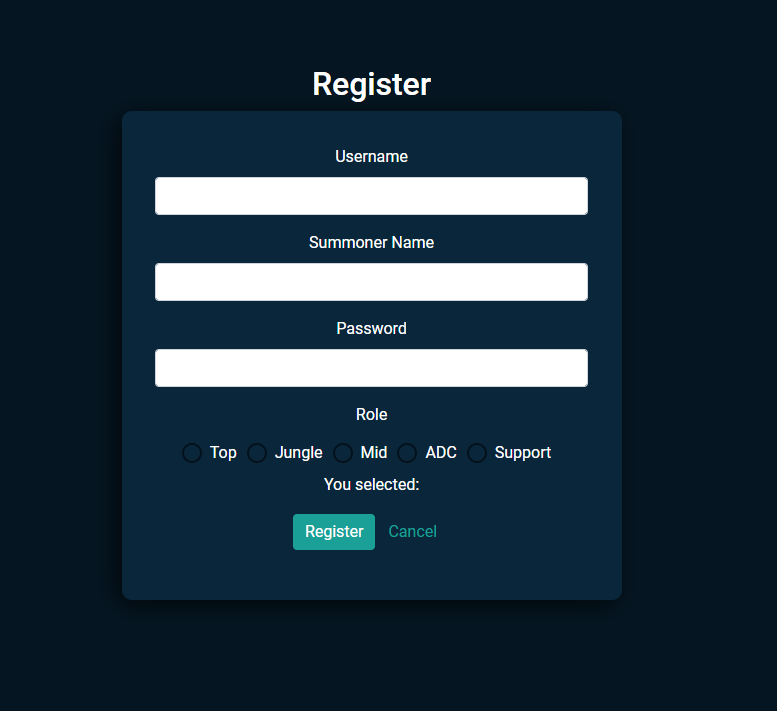
\includegraphics[width=\textwidth/2,height=\textheight/2,keepaspectratio]{img/Register.png}
	\caption{Registration}
	\label{tikz:reg}
	\centering
	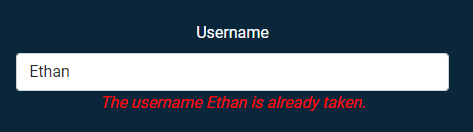
\includegraphics[width=\textwidth/2,height=\textheight/2,keepaspectratio]{img/UsernameTaken.png}
	\caption{Username Taken}
	\label{tikz:taken}
	\centering
	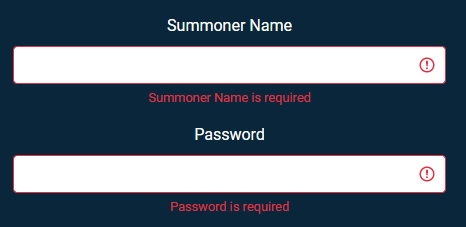
\includegraphics[width=\textwidth/2,height=\textheight/2,keepaspectratio]{img/RequiredFields.png}
	\caption{Required Fields}
	\label{tikz:fields}
\end{figure}


\newpage
\subsection{User Authentication}

\begin{figure}[H]	
	\centering
	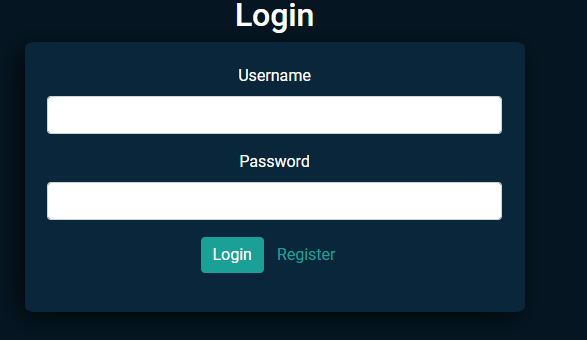
\includegraphics[width=\textwidth/2,height=\textheight,keepaspectratio]{img/Login.png}
	\caption{User Login}
	\label{tikz:login}
	\centering
	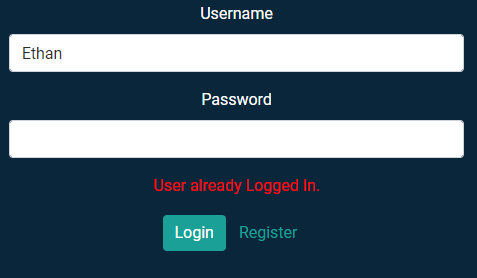
\includegraphics[width=\textwidth/2,height=\textheight,keepaspectratio]{img/LoggedIn.png}
	\caption{Logged In}
	\label{tikz:loggedin}
\end{figure}

User Authentication is responsible for verifying that the user exists and checks if the credentials entered are correct. When the user attempts to log in, the system checks the username to confirm that the user is not already logged in. The client sends a request to the server which first, verifies that the user exits and then the system compares the password entered with the password stored in the database. The user gains access if all the steps mentioned above are acceptable.\hfill \break
The authentication system stores the username in local storage \cite{casario2011html5}; local storage saves key and value pairs in a web browser. Local storage has no expiration date; meaning the user will remain logged in until they log out of the application. Local storage allowed username references throughout the web pages of the application. The system can use the username currently stored in local storage to access more information on that user, like their in-game name or total games.

\subsection{Available Games}


\begin{figure}[H]	
	\centering
	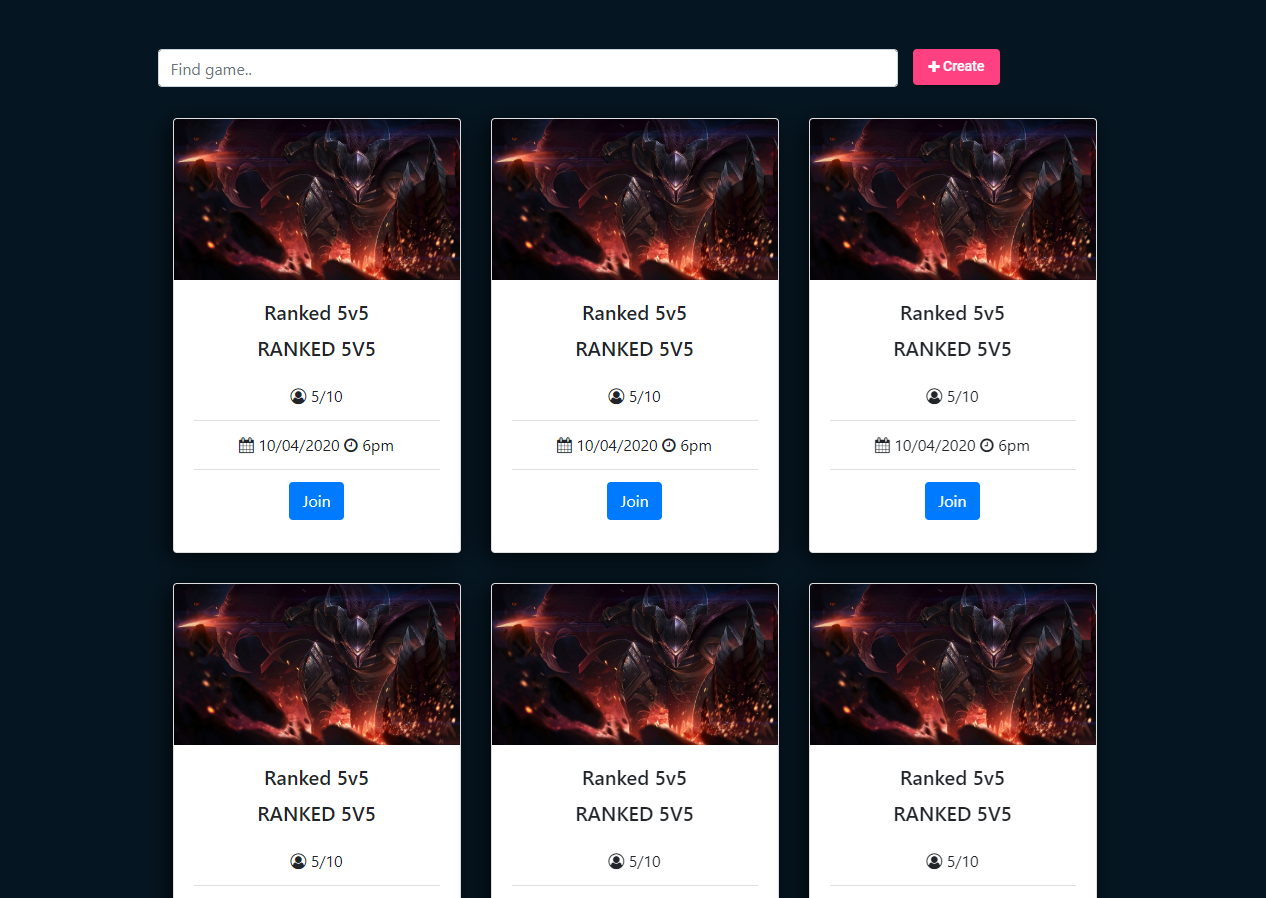
\includegraphics[width=\textwidth,height=\textheight,keepaspectratio]{img/ViewGames.png}
	\caption{Games View}
	\label{tikz:viewgames}
	\centering
	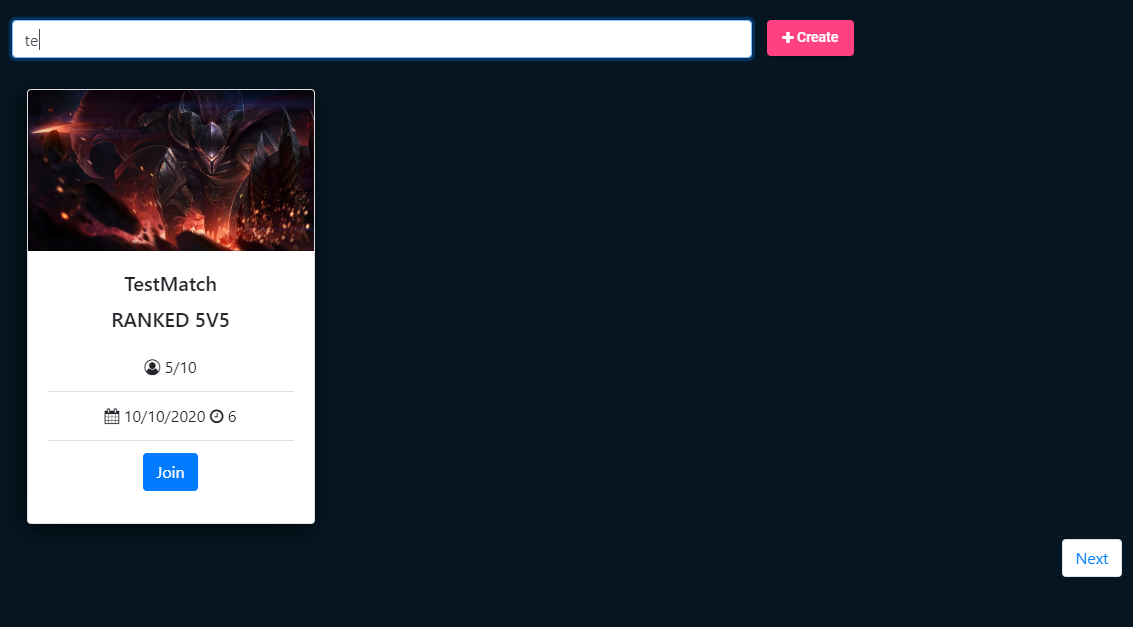
\includegraphics[width=\textwidth,height=\textheight,keepaspectratio]{img/SearchGames.png}
	\caption{Searching for a game}
	\label{tikz:searchgame}
\end{figure}
The available games page contains all the available matches which a user can view or join. The client sends a request to the server to retrieve games that are currently open to the public. If a player wants to find a specific game, they can use the search bar which filters the games to the user's search query, as shown in figure \ref{tikz:searchgame}.


\subsection{Matches}

The matches page contains details for a specific game; When a game is created, the server generates a universally unique identifier (UUID) for each game to distinguish between them. The UUID is used for generating unique pages for every game that is created. We can use python's UUID to achieve this; the function generates a UUID from a host ID, sequence number, and the current time \cite{pythonuuid}. \hfill \break
The matches page displays the time and dates for when the match will take place and the current players that have joined that match. When the number of participants reaches a capacity of 10 players, the matchmaking system will form teams based on the participants and their rating.
\begin{center}    
	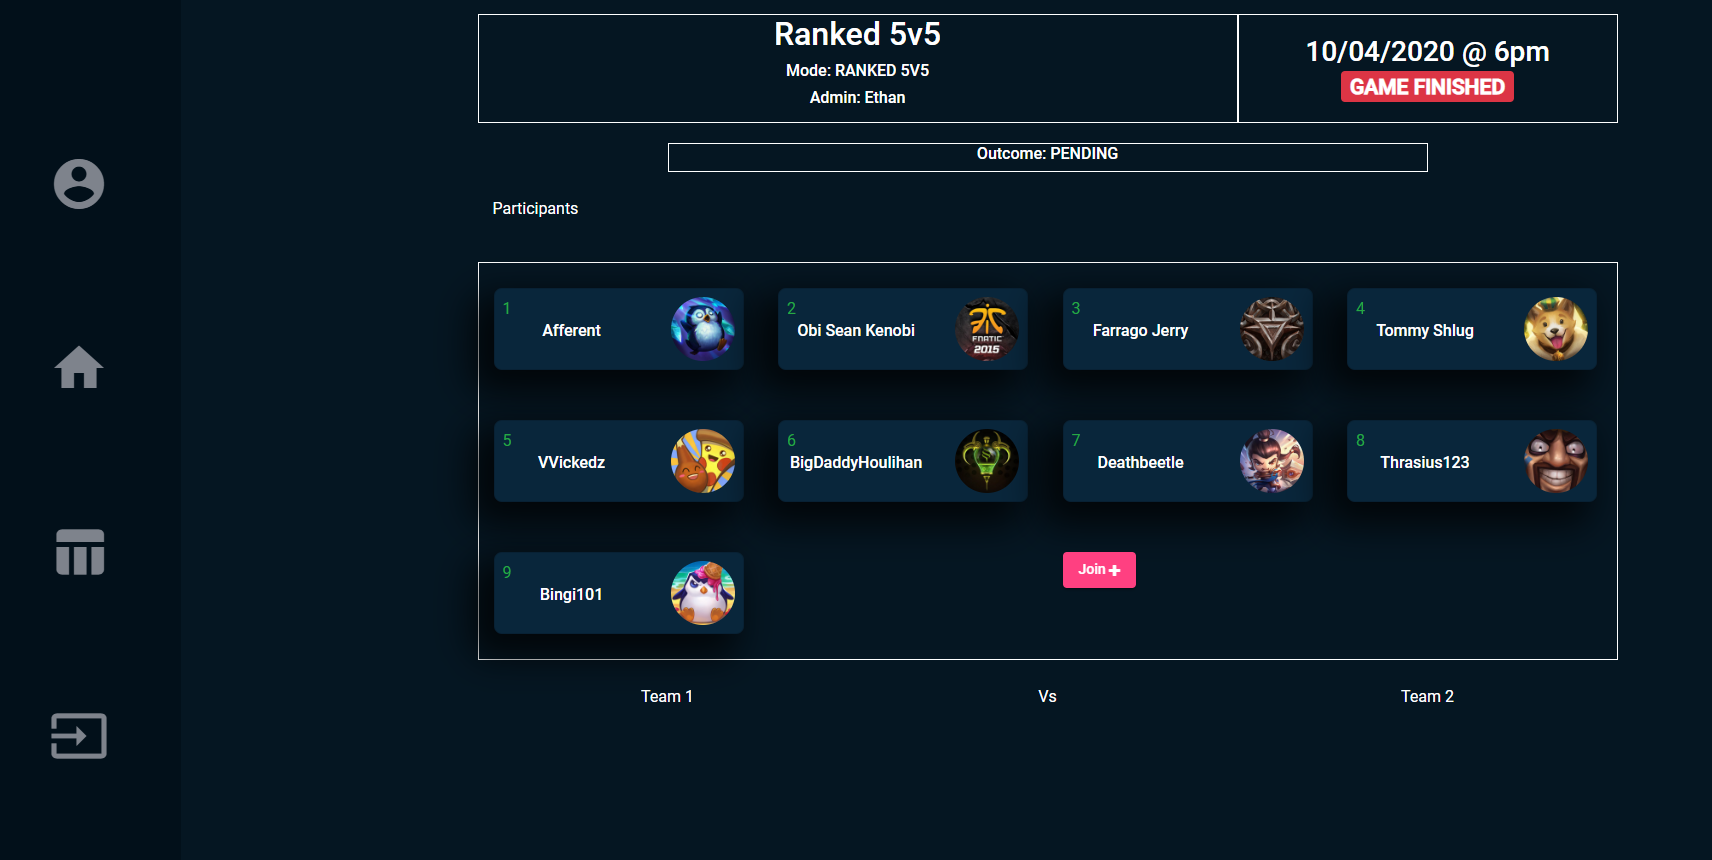
\includegraphics[width=\textwidth,height=\textheight,keepaspectratio]{img/ViewMatch.png}
\end{center}

\subsection{Leaderboards}
The leaderboards page tracks the information of the user based on the games they have played using this platform; it displays their total points, total wins and total losses. The users are placed on the leaderboards based on the number of points they have accumulated. The leadboards aim to generate a competitive environment for the players and also allow players to track their progress, making it easier for players to manage their games.
\begin{center}    
	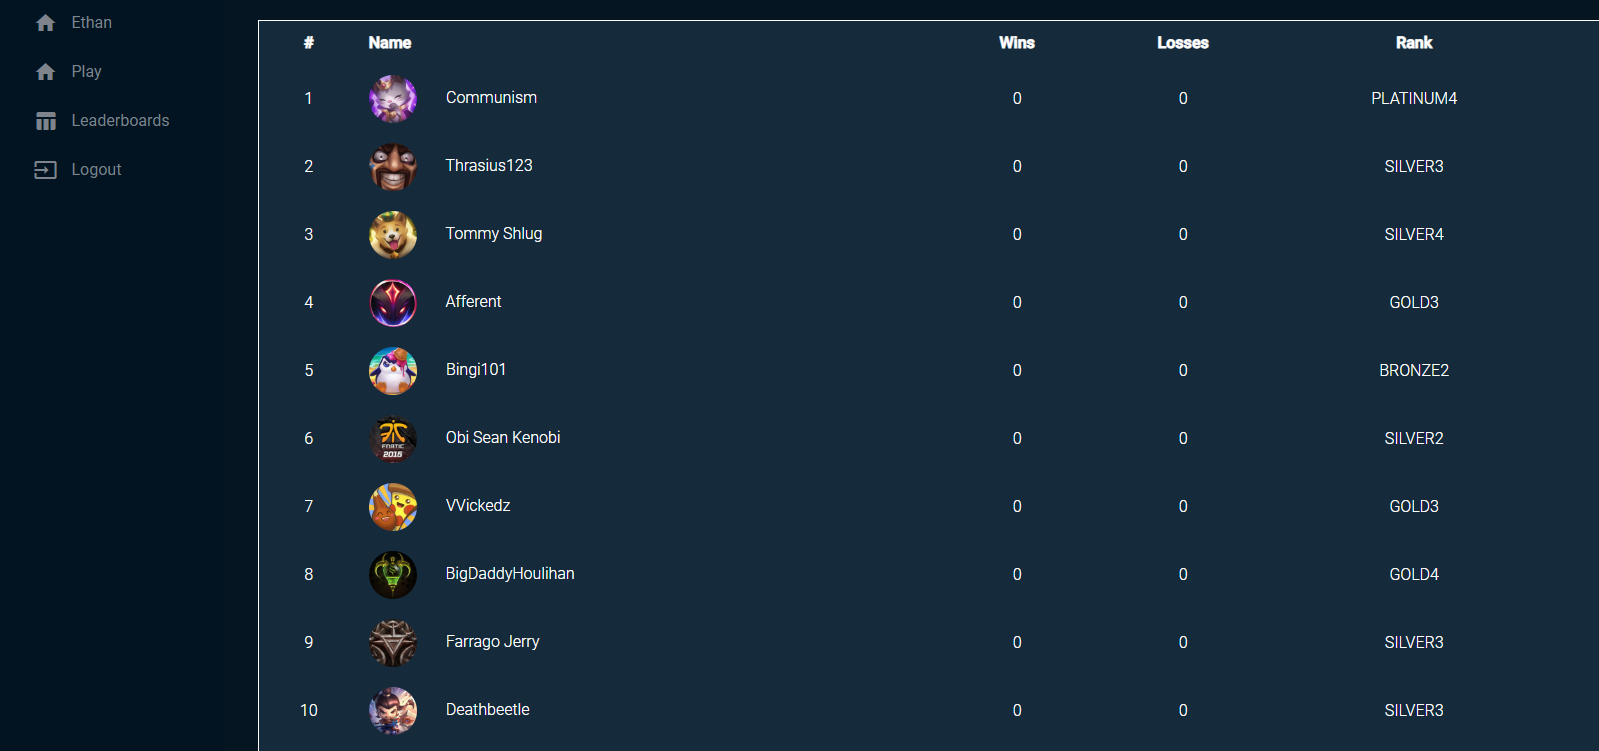
\includegraphics[width=\textwidth,height=\textheight,keepaspectratio]{img/Leaderboards.png}
\end{center}

\newpage
\section{Database Design}

\begin{itemize}
	\item User Table
\end{itemize}
The user table contained the majority of information for the user. This data was a mixture of registration details and their in-game data details.
\begin{table}[h]
	\centering
	\begin{tabular}{ll}
		\toprule
		Column         & Data Type \\
		\midrule
		user\_id       & int       \\
		summoner\_name & varchar   \\
		username       & varchar   \\
		password       & varchar   \\
		rank           & int       \\
		mmr            & int       \\
		total\_games   & int       \\
		primary\_role  & varchar   \\
		account\_id    & varchar   \\
		player\_icon   & int   \\ 
		\bottomrule  
	\end{tabular}
\caption{The user table.}
\end{table}

\begin{itemize}
	\item Participant Table
\end{itemize}
This held data for the players that joined a certain game.
\begin{table}[h]
	\centering
	\begin{tabular}{ll}
		\toprule
		Column         & Data Type \\
		\midrule
		match\_uuid    & varchar   \\
		username       & varchar   \\
		summoner\_name & varchar   \\
		player\_icon   & int       \\
		mmr            & int   \\
		\bottomrule    
	\end{tabular}
\caption{The participant table.}
\end{table}

\newpage
\begin{itemize}
	\item Rank Table
\end{itemize}
The rank table contained all ranks and their MMR equivalent which is used throughout the application and matchmaking.
\begin{table}[h]
	\centering
	\begin{tabular}{ll}
		\toprule
		Column         & Data Type \\
		\midrule
		rank   & varchar   \\
		mmr    & int    \\
		\bottomrule    
	\end{tabular}
	\caption{The rank table.}
\end{table}

\begin{itemize}
	\item Matches Table
\end{itemize}
This table contains all matches that have been created and the status of each match.
\begin{table}[h]
	\centering
	\begin{tabular}{ll}
		\toprule
		Column         & Data Type \\
		\midrule
		match\_uuid & varchar   \\
		match\_name & varchar   \\
		match\_type & varchar   \\
		date        & date      \\
		time        & varchar   \\
		outcome     & varchar   \\
		admin       & varchar   \\
		\bottomrule    
	\end{tabular}
	\caption{The matches table.}
\end{table}

\newpage
\begin{itemize}
	\item Final Match Table
\end{itemize}
When a match reaches its maximum amount of participants, all the participants for a that match are put through the matchmaking algorithm and then stored here. 
\begin{table}[h]
	\centering
	\begin{tabular}{ll}
		\toprule
		Column         & Data Type \\
		\midrule
		match\_uuid & varchar       \\
		team1       & varchar array \\
		team2       & varchar array \\
		\bottomrule    
	\end{tabular}
	\caption{The final match table.}
\end{table}

\section{Algorithms}
For the matchmaking system, I used the Elo System and adapted concepts from the Gale-Shapley algorithm, for the system to work, I first needed the ratings of each participant for a given match. The results I got when accessing Riot's API were presented in this format:\hfill \break
\begin{minted}{json}
	{
	"leagueId": "50bd22e7-16e5-4fe1-bc4a-e364d2a6b124",
	"queueType": "RANKED_SOLO_5x5",
	"tier": "GOLD",
	"rank": "III",
	"summonerId": "<id>",
	"summonerName": "<Username>",
	"leaguePoints": 50,
	"wins": 40,
	"losses": 24,
	}
\end{minted}

The $rank$ and $tier$ is the players rating, I normalized this rating into its integer equivalent, by comparing it to a table I created of constant values.
Since the $rank$ given is in roman numeral format, I created a function which converted roman numerals to integers and then combined the $tier$ with the $rank$ into one string.\hfill \break

Example, $tier: "GOLD"$, $ rank: "III"$ is then converted to $GOLD3$

\newpage
Once the players rating retrieved from Riot Games API converted into one string, I could then compare it to the table of constant values which represents ratings as integer values.

\begin{minted}{python}
[
	"BRONZE4": 100,
	"BRONZE3": 200,
	...
	"SILVER4": 500,
	...
	"GOLD4": 900,
	"GOLD3": 1000
]
\end{minted}
\hfill \break
This procedure occurs every time a user registers with the application; The reasoning behind this is to try and minimize the time needed for the matchmaking system to form teams.\hfill \break
I wanted to improve the Matchmaking system to generate more balanced teams.
To achieve this, I calculated the growth rate \cite{d2010production} for players; this growth rate determined how long it took for a given player to reach that rating, if player $a$ got the same rank as player $b$ in a shorter period, then it is assumed that player $a$ is performing better than player $b$.

\begin{figure}[H]
	\centering
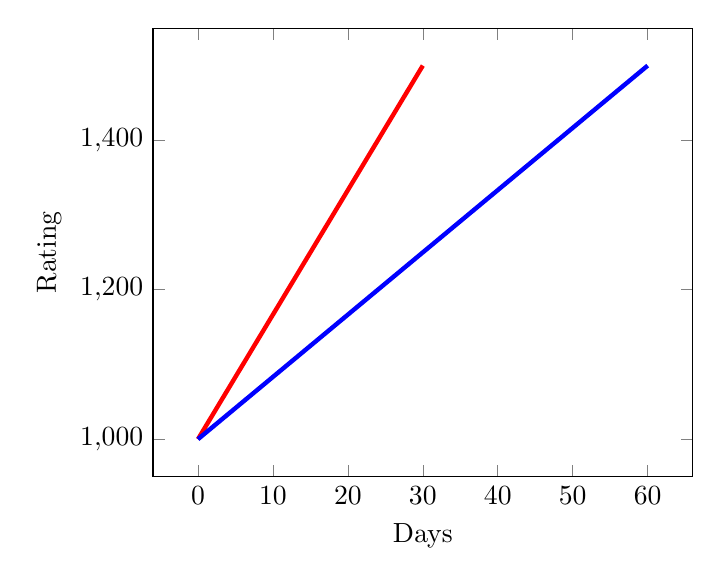
\begin{tikzpicture}
\begin{axis}
       [
xlabel={Days},
ylabel={Rating}
]
\addplot [mark=none,  red,   ultra thick] coordinates { (0,1000) (30, 1500)};
\addplot [mark=none,  blue,   ultra thick] coordinates { (0,1000) (60, 1500)};
\end{axis} 
\end{tikzpicture}
	\caption{Growth Rate Example}
	\label{tikz:growth}
\end{figure}

\newpage
Say we have player $a$ with a rating $RP$ and an initial rating $RS$.
We can calculate growth rate $g$ with: 
\[ g = \frac{\frac{(RP - RS)}{RS} \times 100}{n} \] 
Where $n$ is the amount of games played to receive that rank.\hfill \break
Then to calculate the players new rating $NR$ we just add the growth rate and current rating.
\[ NR = \frac{\frac{(RP - RS)}{RS} \times 100}{n} + RP \]

This growth rate is used in cases when trying to matchmake multiple players with the same rating.\hfill

\paragraph{For Example:} If we had four players with the same rating of 900 but they each got that rating in a different amount of games, we can match them based on their rating + growth rate.

\[ player A = \frac{\frac{(900 - 500)}{500} \times 100}{15} + 900 = 905.3 \]
\[ player B = \frac{\frac{(900 - 500)}{500} \times 100}{50} + 900 = 901.6 \]
\[ player C = \frac{\frac{(900 - 500)}{500} \times 100}{30} + 900 = 902.6 \]
\[ player D = \frac{\frac{(900 - 500)}{500} \times 100}{26} + 900 = 903.1 \]

Therefore, we would match $player A$ vs $player D$ and $player B$ vs $player C$

\subsection{The Elo System}
The Elo rating system, developed by Arpad Elo, is used for calculating relative skill levels of players in games such as chess.\cite{glickman1999rating} A rating is a number normally between 0 and 3000, this number changes depending on the outcomes of games. When a players rating is unknown, the score for a player is assumed to be:
\[ E_a = \frac{1}{1+10\frac{E_a-E_b}{400}} \] \cite{pelanek2014application} A player's change in rating is calculated by the following formula where ${S_a}$ is the result of the game (${Win = 1}$ and $Loss = 0$), $R_o$ is the old rating and $R_n$ is the new rating.
\[ R_n = R_o + K(S_a - E_a) \]


{\raggedright The size of the score change is determined by a dynamic K value. Initially, this K value is big (30 for their first 30 games) resulting in rapid changes in Elo. This is so a player can quickly find his or her correct place in the ranking system. As the number of games increases the K value is reduced to prevent dramatic changes in Elo.}\newline
\cite{glickmanrating} The value K used to take on the values 32, 24 or 16, depending on a player’s pre-event rating. K Factor can also be defined through this equation, where $N_i$ is the effective number of games, and m is the number of games the player completed in the game.
\paragraph{Example} If Player $E_a$ has a rating of 1200 and Player $E_b$ has a rating of 1000 with both having a K value of 30, Player $E_a$ is expected to win. If Player $E_b$ wins, the rating for player $E_b$ will increase more compared to if $E_a$ won because its rating is higher.\vfill

\subsection{Gale Shapely Algorithm}
The Gale-Shapely algorithm \cite{dubins1981machiavelli} is an algorithm for the stable matching problem. \cite{gale1985some}


David Gale and Lloyd Shapley proved that \cite{gale1962college}, for an equal number of men and women, it is possible to make all marriages stable. 

\paragraph{}
The algorithm involves different rounds.

\begin{itemize}
	\item Round 1
\end{itemize}
All single men propose to the woman he favours most.
\begin{itemize}
	\item Round 2
\end{itemize}
Each woman is then temporarily taken by the suitor she most prefers so far, and that suitor is likewise provisionally engaged to her.
\paragraph{In each following round:}
\begin{itemize}
	\item a
\end{itemize}
All unengaged men propose to their most-preferred woman (even if the woman is already "engaged" )
\begin{itemize}
	\item b
\end{itemize}
If a woman prefers this man over her current temporary partner, they become unengaged and the woman and new man become "engaged".
This process is repeated until everyone is engaged.

\paragraph{In the end}
\begin{itemize}
	\item Everyone gets married.
\end{itemize}
There can't be a people unengaged.\newline 
\begin{itemize}
	\item The marriages are stable.
\end{itemize}
Say, we have a woman and man that both have their partners, Let's call them Mary and John.
When the algorithm is finished, both Mary and John can't prefer each other over their current partners. If John prefers Mary to his current partner, he must have already proposed to Mary before he proposed to his current partner. If Mary accepted his proposal, yet is not married to him at the end, she must have gone for someone she prefers more and therefore doesn't like John more than her current partner. 

\newpage
\section{Microservices}
\begin{center}    
	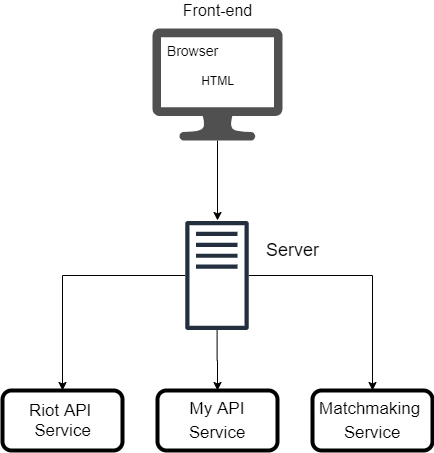
\includegraphics[width=\textwidth/2,height=\textheight/2,keepaspectratio]{img/Microservice.png}
\end{center}
Microservices is an architecture style which separates the system into individual services that build a cohesive system. \cite{alshuqayran2016systematic} I used this architecture style for communication integration. I created a service for connection with Riot Games API and different service for communication with the applications API, both these services then communicated with the projects database for further usage during development. This style provided portability \cite{dragoni2017microservices} since each service was loosely coupled \cite{salah2016evolution}, meaning I could access these classes independently, not only did this give a more fluent workflow, it made life a lot easier when conducting tests.
Companies like Netflix \cite{bukoski2018we} make use of microservices to allow their teams to "build and push at comfortable speeds".
\newpage
\subsection{Data Communication}
Interfacing with Riot Games API was vital for the system to function, Riot's API stored the user's in-game details which were needed to gain information on player ratings, players usernames and players in-game statistics.\hfill \break 
Riotwatcher \cite{riotwatcher}; a python wrapper for riot games API was used to perform requests to Riots API.\hfill \break
For Example, to retrieve players the total amount of games, we would execute this function:
\begin{minted}{sql}
def get_total_games(self):
	account_id = Summoner.get_account_id(self)
	wins = watcher.league.by_summoner(my_region, account_id)
	total_games = wins[0]['wins'] + wins[0]['losses']
	return total_games
\end{minted}
We store similar data like the players rating and various other information in the database of the application, with this information in the application's database allowed for further manipulation and usage throughout the project, such as the matchmaking system. Without external API's like Riot's API, the application would not fully work as intended, without player ratings the matchmaking system would be very inaccurate due to the fact we would have to predict player ratings to some extent.\hfill \break 
The functionality of accessing API's was kept generalized as possible to future proof it allowing more game platforms to be added.\hfill \break 
\bigskip

\subsection{Limiting}
Retrieving the player's details from riot's API is only performed once during registration, and updated each time a user logs in, the reason for this is to limit the number of calls made to riot's API due to its rate-limiting restrictions; rate-limiting manages the volume of incoming and outgoing traffic to or from a network \cite{raghavan2007cloud}. For example, riots API service allows 100 requests/minute. If the number of requests exceeds that limit, then an error will occur.

\newpage
\section{Testing Design}
When designing tests for the application, the main objective was to cover the system at the internal logic level and user level. Software tests identified errors and the quality of the software \cite{nidhra2012black} to produce a robust system. Two different approaches were used to test the application, white-box testing and black-box testing. 
\begin{itemize}
	\item White-box testing: A detailed investigation of internal logic and structure of the code. In white-box testing, a tester must have full knowledge of the source code.
	\item Black-box testing: A testing approach without having any knowledge of the software's internal workings, it examines components of the application at the user level.
\end{itemize}

The core testing frameworks used throughout the project were Jasmine, Protractor, Python's Unit Test and Selenium. 
\subsection{Front-end Testing}
When testing the front-end of the application, we use white-box and black-box testing approaches. The test cases written in protractor performed end-to-end tests (e2e).e2e tests simulate real user scenarios and the flow of the system. e2e tests verified that the elements of the web pages displayed accurately and that the intention was correct.
Here is an example of an e2e test case which verifies that the heading on the given page is correct.
\begin{minted}{javascript}
it('should open create page', () => {
	page.navigateToPage(browser.baseUrl);
	page.getCreateButton();
	expect(browser.getCurrentUrl()).toMatch('/creategame')
});
\end{minted} 

\chapter{System Evaluation}
\section{Limitations}
\subsection{Limited Data Access}
One of the main limitations of this project is not being able to gain access to data for custom games. The main aim of this project was to automate the process of managing custom matches and not being able to gain access to the outcome of these matches within Riots API, indicated that someone or something is responsible for determining the result of a game. To remedy this, the application creates an administrator based on the organiser of the match, he/she is responsible for confirming the outcome of a game, although this can raise multiple potential problems. I can not think of another way to combat this issue.
\newpage
\subsection{API Key}
The API key to access Riot Games API changed every day, this meant each day I was working on the project, I'd have to regenerate a new API key. After I created a new API key, I could not access the API immediately, I would have to wait a while before being able to access it again. The only way to get a static API key is to submit your application for review by Riot Games and hope they approve, this was also an extra limitation as they would not accept applications currently in development. Therefore, there was no way for me to receive a static API key. Although this is not a significant limitation, it's more of a minor inconvenience.
\subsection{Tournament Codes}
Riot Games can supply tournament codes, which would have given me the capabilities of creating custom games where the player needs a key to access. Gaining access to tournament codes would have suited the system a lot because I could then gain access to information about these games and their outcomes, meaning the application's process of managing matches would be automated other than creating and signing up. The only way to receive these tournament codes was to make the custom matches on the application, prized events, meaning the winners of a match would receive some form of prize. Although this is a minor drawback, I still created a workaround which can be a temporary solution until I acquire a production API key.
\subsection{Software Dependent}
Software reliability is defined as the probability of failure-free software development for a named period in a specified environment \cite{huang2007assessment}. Since this project is a service for online games, the application depends on third-party software such as riot games API to function, and will only operate when the third-party software is also working. 

For example, if the game servers go down for a period, then nobody can use this application because the servers are down, denying them access to play the game. The best option for this would be to combine multiple online games into the app instead of being restricted to just one, genres like first-person shooters and strategy games could effortlessly be implemented because they follow universal rating systems. Adding more games to the platform would ensure that the project will always have some form of usability.\hfill \break

Another reason this project is software dependent is because of its use of external API's.
Third-party API's always change, meaning this application has to match any changes the third-party API makes. Functionality can be also be refactored or deprecated, possibly remodelling the purpose of its intended use. \hfill \break
Alternatives like web scraping are additional options I could use to obtain data on players in-game details. Web scraping is a process of automatic data collection from the internet, commonly in website pages using markup languages such as HTML \cite{slamet2018web}. Although web scraping might seem like a viable option, the web sites that I could gather data from may also be reliant on third-party software which circles back to the dilemma stated above.
\section{Vulnerabilities}
When migrating the database over to PostgreSQL, I stumbled upon a vulnerability in how I was handling requests and insertions in my database. My queries were not parameterized meaning attackers could potentially harm my database, by deleting tables or even releasing sensitive information. This is commonly referred to as SQL Injection. 

The types of attacks that could have been performed on my old procedures are called "Piggy-Backed Queries" \cite{halfond2006classification}, in this type of attack, the attacker will attempt to add an extra query to the original query. 
\newline Piggy-Backed query example:

\begin{minted}{sql}
SELECT username FROM users WHERE login=john; drop table users;
\end{minted}

After executing the above query, the database will recognise the semicolon (';') which determines the end of the first query, the second query is the injected query which would destroy the table, removing any valuable data within.

\paragraph{}
SQL injection \cite{halfond2006classification} can cause an obvious threat to web applications, they enable attackers to modify queries and even release sensitive information (i.e passwords).

To solve this potential vulnerability, I ensured that all my queries were parametrized \cite{psycopg}.
\begin{minted}{python}
p_query = ("insert into participants values(%s, %s, %s, %s, %s)")
p_param = (_match_uuid, _username, _summoner_name, _player_icon, _mmr)
\end{minted}
I also assured the only data that the user could enter were alphanumeric characters: no symbols were allowed.

Writing Secure Code\cite{howard2003writing} by Michael Howard and David LeBlanc is an interesting read that provides good practices for writing secure code and SQL queries.

\section{Robustness}
To ensure my system was robust I conducted multiple types of tests, including:

\begin{itemize}
	\item Back-end Unit Testing.
	\item Front-End Unit Testing.
	\item e2e Testing.
	\item Automated Testing.
\end{itemize}

Theses tests were responsible for testing various different components of the project, unit tests were added to test individual components, I tried to emulate how a real-world user would use the system through automated tests.\newline
Incorporating multiple tests allowed me to discover errors that may not have been found. Testing at multiple layers of the application ensured that the system was robust.
\chapter{Conclusion}
I set out to develop an application that could automate the organisation of custom matches with the intent of making it more manageable for people to run their events, focusing on the end goal and researching various concepts related to this application enabled me to achieve this goal. This project was no simple task, but yet it was satisfying and valuable; I feel I've got more insight into how real-world applications are developed.  Although I could not automate the process of accessing match outcomes which I discussed above, I consider the alternative solution a viable option. In the future, I aim to submit this application to Riot Game's API for review so I can gain access to tournament codes, which opens up more opportunities for me to scale this application. Being in a group of friends and acquaintances that also play similar games motivated me to develop this system.


\subsection{Opportunities}
Throughout development and on completion, I discovered potential opportunities, including an API for custom online events, such as matches and tournaments. Instead of being restricted to the web application, people could integrate this API into their application or system. I could develop a python package with the implementation of the Elo System; this would be a useful resource for developers who are creating their own game and require some form of rating system for their players.
I could potentially scale this application by incorporating multiple online game platforms, which would significantly increase the size of the platform, and similar concepts of matchmaking are still applicable. I'd incorporate a tournament system in the style of knockout stages; this would further increase the competitive environment.

\subsection{What would I do differently?}

In hindsight, there are various things I would have done differently:
\begin{itemize}
	\item Use some form of project management from the very beginning.
	\item Travis CI for continuous integration, which would help greatly with developing and testing in smaller increments and also automate parts of the development process by managing deployments.
	\item Deploy at the Beginning.
	\item Decide on a database before even starting development, I was unsure if i should have used an SQL database or a NoSQL database, I auditioned both and in the end I chose SQL, I could have saved some valuable time if I decided on a database at the very beginning.
	\item Test more and Test early, I only started testing towards the end of development which was very tricky, if I were to develop this application again, I would incorporate tests for any new element that was added.
\end{itemize}

If I were to rework some components of this application, the user authentication system would be the first. Instead of using my authentication system, I would integrate a third-party system. I would do this from a security standpoint; the benefits of using a third-party system is that they would handle all the authentication processes for me while also being secure. Firebase provides this functionality, which is convenient because it is the same platform that the frontend of this application is deployed. The third-party authentication would also go hand-in-hand with the possible public API that I mentioned above because I could separate the sensitive information with the public information.

